\documentclass[11pt,a4paper]{ivoa}
\input tthdefs

\usepackage{listings}
%\lstloadlanguages{sh,make,xml,[latex]tex}
\lstset{flexiblecolumns=true,numberstyle=\small,showstringspaces=False,
  identifierstyle=\texttt,defaultdialect=[latex]tex,language=tex}


\title{IVOA Single-Sign-On Profile: Authentication Mechanisms}

\ivoagroup{http://www.ivoa.net/twiki/bin/view/IVOA/IvoaGridAndWebServices}

%\author[????URL????]{http://www.ivoa.net/twiki/bin/view/IVOA/IvoaGridAndWebServices}
\author{Brian Majour, Guy Rixon, Andr\`e Schaaff, Giuliano Taffoni}

\editor{Giuliano Taffoni}

\previousversion[http://www.ivoa.net/documents/cover/SSOAuthMech-20080124.html]{REC-1.0}
\previousversion[http://www.ivoa.net/documents/cover/SSOAuthMech-20070904.html]{PR-20070904}
\previousversion[http://www.ivoa.net/documents/cover/SSOAuthMech-20070621.html]{PR-20070621}
\previousversion[http://www.ivoa.net/documents/cover/SSOAuthMech-20060519.html]{WD-20060519}
       

\begin{document}
\begin{abstract}
Approved client-server authentication mechanisms are described for the IVOA single-sign-on profile: No Authentication; HTTP Basic Authentication; TLS with passwords; TLS with client certificates; Cookies; Open Authentication; Security Assertion Markup Language; OpenID. Normative rules are given for the implementation of these mechanisms, mainly by reference to pre-existing standards. The Authorization mechanisms are out of the scope of this document.
\end{abstract}


\section*{Acknowledgments}

This document derives from discussions among the Grid and Web Services working-group of IVOA. It is particularly informed by prototypes built by Matthew Graham (Caltech/US-NVO), Paul Harrison (ESO/EuroVO), David Morris (Cambridge/AstroGrid) and Raymond Plante (NCSA/US-NVO). The prior art for the use of proxy certificates comes from the Globus Alliance.
This document has been developed with support from the National Science Foundation's Information Technology Research Program under Cooperative Agreement AST0122449 with The Johns Hopkins University, from the UK Particle Physics and Astronomy Research Council (PPARC) and from the Europena Commission's Sixth Framework Program via the Optical Infrared Coordination Network (OPTICON).


\section*{Conformance-related definitions}
The words ``MUST'', ``SHALL'', ``SHOULD'', ``MAY'', ``RECOMMENDED'', and
``OPTIONAL'' (in upper or lower case) used in this document are to be
interpreted as described in IETF standard, \citet{std:RFC2119}.

The \emph{Virtual Observatory (VO)} is
general term for a collection of federated resources that can be used
to conduct astronomical research, education, and outreach.
The \href{http://www.ivoa.net}{International
Virtual Observatory Alliance (IVOA)} is a global
collaboration of separately funded projects to develop standards and
infrastructure that enable VO applications.


\section{Introduction}
IVOA's single-sign-on architecture is a system in which users assign cryptographic credentials to user agents so that the agents may act with the user's identity and access rights. This standard describes how agents use those credentials to authenticate the user's identity in requests to services. This standard describes also the authentication mechanism of an application or a service making a call (on behalf of someone or something else) to an API or to another service.
This document is essentially a {\em profile} against existing security standards; that is, it describes how an existing standard should be applied in an IVOA application to support single sign-on capabilities in the IVOA. In the following sections, we make specific references to details spelled out in these standards. For the purposes of validating against this standard, those referenced documents should be consulted for a full explanation of those details. Unfortunately, a reader that is unfamiliar with these external standards might find this specification confusing. To alleviate this problem, each major section is concluded by a Commentary subsection that provides some explanations of the detailed terms and concepts being referred to. The Commentary subsection may also provide recommended scenarios for how this specification might actually be realised. Note that the statements in the Commentary subsections are non-normative and should not be considered part of precise specification; nevertheless, they are indicative of the intended spirit of this document.

\subsection{Role within the VO Architecture}

\begin{figure}
\centering

% Get the architecture diagram from the TCG chair
% http://wiki.ivoa.net/twiki/bin/view/IVOA/IvoaTCG
% If they give you a PDF, for now dumb it down to a png by
% convert -antialias -density 72x72 archdiag.pdf archdiag.png
% Oh -- Notes don't need this; you'd have to remove archdiag.png
% from FIGURES in the Makefile, too.
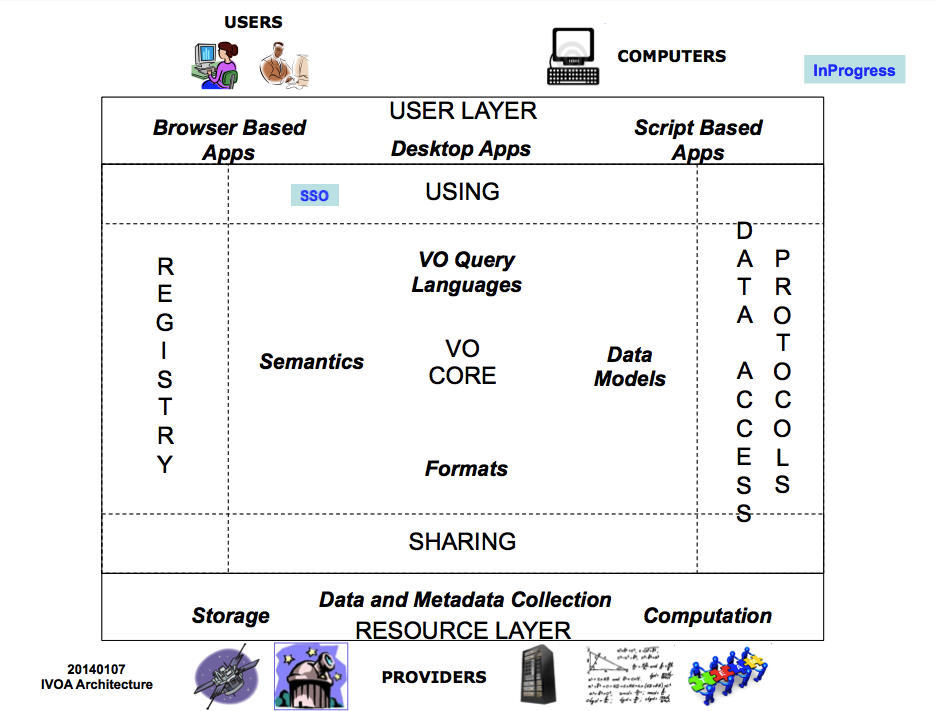
\includegraphics[width=0.9\textwidth]{SSO_image001.png}
\caption{Architecture diagram for this document}
\label{fig:archdiag}
\end{figure}

Fig.~\ref{fig:archdiag} shows the role this document plays within the
IVOA architecture \citep{note:VOARCH}.


\section{Scope of this standard}
\subsection{Requirements}
When a service is registered in an IVOA registry, that services resource document MAY include metadata expressing conformance to one or more of the authentication mechanisms approved in the IVOA SSO profile. Such a service MUST implement those mechanisms as described in this document, and clients of the service MUST participate in the mechanism when calling the service. Is a service does not provide any SSO specification it is assumed that no authentication is required.
The registration of the service interface SHALL contain an XML element
of type \xmlel{SecurityMethod} as specified in the XML schema for
VOResource \citep{std:VOR}. The value of this element distinguishes the
authentication mechanism using the values stated in the sections below.
Services registered without the metadata alluded to above need not
support any authentication mechanism. If they do require authentication,
they MAY use either the IVOA-standard mechanisms or others that are not
IVOA standards.

\subsection{Commentary}
The IVOA SSO profile allows the development of a ''realm'' of interoperable services and clients. 
Service providers opt in to this realm by implementing this current standard and by registering accordingly in the IVOA registry. 
This allows clients to discover a secured service through the registry and to be able to use it without 
being customized for the details of the specific service.

Services within the Virtual Observatory that are not intended to be widely interoperable need not opt in to the SSO realm. 
In particular, ''private'' services, accessed by web browsers and protected by passwords, are allowed. 
However, these private services should be reworked to follow the IVOA standard if they are later promoted to a wider audience.

An example of a registration for a secured interface follows.
\begin{lstlisting}[language=XML]
<interface xmlns:vs='ivo://www.ivoa.net/xml/VODataService/v1.0'  
	xsi:type='vs:ParamHTTP'>
	<accessURL>http://some.where/some/thing</accessURL>
	<securityMethod>ivo://ivoa.net/sso#saml2.0</securityMethod>
</interface> 
\end{lstlisting}

More than one {\xmlel securityMethod} can be specified:
\begin{lstlisting}[language=XML]
<interface xmlns:vs='ivo://www.ivoa.net/xml/VODataService/v1.0'  
	xsi:type='vs:ParamHTTP'>
	<accessURL>http://some.where/some/thing</accessURL>
	<securityMethod>ivo://ivoa.net/sso#saml2.0</securityMethod>
	<securityMethod>ivo://ivoa.net/sso#cookie</securityMethod>
	<securityMethod>ivo://ivoa.net/sso#OpenID</securityMethod>
</interface> 
\end{lstlisting}

The order of the \xmlel{securityMethod} elements determines the priority of the method to use, in the example above the preferred method to access 
the service is {\em SAML}, than {\em cookies} and finally if the other are not available OpenID.

\section{Approved authentication mechanisms}

The following authentication mechanisms are approved for use in the SSO profile.
\begin{itemize}
\item No authentication required.
\item HTTP Basic Authentication
\item Transport Layer Security (TLS) with passwords.
\item Transport Layer Security (TLS) with client certificates.
\item Cookies
\item Open Authentication (OAuth) 
\item Security Assertion Markup Language (SAML) 
\item OpenID 
\end{itemize}

The mechanism is associated with the interface provided by the service and registered in the IVOA registry.
 
\begin{table}[th] \begin{tabular}{p{0.45\textwidth}p{0.64\textwidth}} \sptablerule
\textbf{SSO mechanism}&\textbf{\xmlel{<securityMethod>}}\\ \sptablerule
No authentication required & none\\
 HTTP Basic Authentication &
\xmlel{https://www.w3.org/Protocols/HTTP/ 1.0/spec.html\#BasicAA}\\
TLS with password &  \xmlel{ivo://ivoa.net/sso\#tls-with-password} \\
TLS with client certificate & \xmlel{ivo://ivoa.net/sso\#tls-with-certificate} \\
Cookies & \xmlel{ivo://ivoa.net/sso\#cookie} \\
Open Authentication & \xmlel{ivo://ivoa.net/sso\#OAuth} \\
SAML &  \xmlel{ivo://ivoa.net/sso\#saml2.0} \\
OpenID &  \xmlel{ivo://ivoa.net/sso\#OpenID} \\
\sptablerule
\caption{List of approved authentication mechanisms and the corresponding securityMethod}
\label{table:SMtable}
\end{tabular}
\end{table}

Services that are registered with a IVOA registry as having a {\em WebService} type interface 
\citep{ivo:resource} SHALL support OAuth, or SHALL support cookies or SHALL support TLS with client 
certificates or SHALL require no authentication.
Interfaces by which a user logs in to the SSO system SHALL support either 
TLS with client certificates, or TLS with passwords, or SAML or a combination of  them

\section{HTTP Basic Authentication}
\subsection{Requirements}
Services using HTTP basic authentication SHALL use the authentication mechanism described in the RFC7235 \citep{std:RFC7235}
that updates RFC2617  \citep{std:RFC2617}. 
Interfaces using this mechanism SHALL be be registered with the security method 

 \texttt{https://www.w3.org/Protocols/HTTP/1.0/spec.html\#BasicAA}

\subsection{Commentary}
HTTP provides a simple challenge-response authentication framework that can be used by a server to challenge 
a client request and by a   client to provide authentication information.
The HTTP authentication framework does not define a single mechanism for maintaining the confidentiality of credentials. 
HTTP depends on the security properties of the underlying transport-   or session-level connection to provide 
confidential transmission of   header fields. Connection secured with TLS are recommended prior to exchanging any credentials.

\section{Details of TLS}
\subsection{Requirements}
Services using Transport Layer Security (TLS) SHALL do so according to the TLS v1.2 standard RFC5246 \citep{std:RFC5246}.

\subsection{Commentary}
TLS supersedes the Secure Sockets Layer that is an outdated cryptographic protocol.   
TLS v1.0 was based on SSL v3.0; the current version of TLS is V1.2 described in by \citet{std:RFC5246}.  
TLS v1.2 is backwards compatible with TLS v1.0, TLS v1.1 and SSL v3.0. 
``TLS versions 1.0, 1.1, and 1.2, and SSL 3.0 are very similar, and use compatible ClientHello messages; 
thus, supporting all of them is   relatively easy.[...] TLS 1.2 clients that wish to support SSL 2.0 servers MUST 
send  version 2.0 CLIENT-HELLO messages defined in SSL2.'' \citep{std:RFC5246}.

\section{Details of TLS-with-client-certificate}
\subsection{Requirements}
Certificates SHALL be transmitted and checked according to the TLS v1.2 standard RFC5246.

Services implementing TLS MUST support certificate chains including proxy certificates according to RFC6818  \citep{std:RFC6818}.

Interfaces using this mechanism SHALL be be registered with the security method 

\texttt{ivo://ivoa.net/sso\#tls-with-certificate}.

\subsection{Commentary}
When Mutual Certificate Authentication is configured for REST services, both, the client and the service perform 
identity verification or authentication through X.509 certificates. 

The client authenticates the service during the initial SSL handshake, when the server sends the client a certificate to authenticate itself.

\section{Details of TLS-with-password}
\subsection{Requirements}
The user-name and password SHALL be passed in the message protected by the TLS mechanism, 
not as part of the mechanism itself. The ``HTTP basic authentication'' should be used with particular attention.

Interfaces using this mechanism SHALL be be registered with the security method 

\texttt{ivo://ivoa.net/sso\#tls-with-password}.

\subsection{Commentary}
``HTTP basic authentication'' passes the user-name and password in the HTTP headers, 
assuming that the credentials are not a natural part of the message body. 
This standard applies the TLS-with-Password mechanism only to the special case of logging in to the SSO realm. 
Hence, the user name and password are logically part of the message body, not the message header.

\section{The use of Cookies}
\subsection{Requirements}
Cookie-Based Authentication uses server side cookies to authenticate the user on every request. 
The way to manage  cookies for authentication is described in RFC6265 \citep{std:RFC6265}.

Interfaces using this mechanism SHALL be be registered with the security method 

\texttt{ivo://ivoa.net/sso\#cookie}.


\subsection{Commentary}
RESTful web services should use session-based authentication, either by establishing a session token via a POST or
by using an API key as a POST body argument or as a cookie. 
User names, passwords, session tokens, and API keys should not appear in the URL, 
as this can be captured in web server logs, which makes them intrinsically valuable.
\begin{figure}
\centering
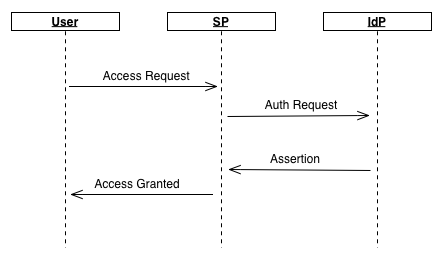
\includegraphics[width=0.9\textwidth]{SSO_image002.png}
\caption{Simplified picture of SAML 2.0 authentication.}
\label{fig:saml}
\end{figure}

\section{Details on SAML authentication}
\subsection{Requirements}
Services using SAML authentication mechanisms SHALL do so according to the 
saml-core-2.0-os OASIS standard \citep{std:SAML}. 
SAML includes protocols and protocol bindings and security \citep{std:SAMLB}.

Interfaces using this mechanism SHALL be be registered with the security method 

\texttt{ivo://ivoa.net/sso\#saml2.0}.


\subsection{Commentary}
SAML presumes two primary roles in any transaction: the organisation where the identity is established, 
known as the Identity Provider (``IdP''), or Asserting Party (``AP''); 
and the organisation which (for this transaction) wants to use this identity, known as the Service Provider (``SP''), 
or Relying Party (``RP'').

A user attempts to access an application with the Service Provider. 
The SP needs to establish the identity of this user, and so sends an authentication request to the Identity Provider. 

The user authenticate with the IdP (IdP is taking care of the authentication mechanisms and protocols e.g. Kerberos, ldap etc.) so the IdP can send back an `Assertion' to the SP. 
Now the SP knows who the user is, and can process that user accordingly (see Fig.~\ref{fig:saml}).
\begin{figure}
\centering
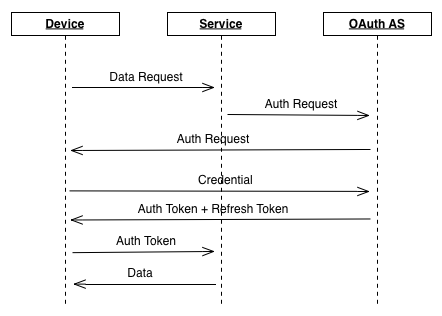
\includegraphics[width=0.9\textwidth]{SSO_image003.png}
\caption{Simplified picture of OAuth 2.0 authentication.} 
\label{fig:oauth}
\end{figure}
 
SAML2.0 protocol allows also to implement authentication service discovery mechanisms. SAML2.0  defines a browser-based protocol 
by which a centralized discovery service can provide a requesting service provider with the unique identifier of an 
identity provider that can authenticate a principal. In this way 


\section{Details on OAuth}
\subsection{Requirements}
Services using OAuth authentication mechanisms SHALL do so according to the RFC6749 \citep{std:RFC6742}.

Interfaces using this mechanism SHALL be be registered with the security method 

\texttt{ivo://ivoa.net/sso\#OAuth}.


\subsection{Commentary}
Open Authentication 2.0 (also in conjunction with OpenID Connect) is actually the adopted standard 
to handle identity in the framework of RESTful web services. 
OAuth is used when an application is making a request on behalf of a user.

OAuth introduces the notion of an `authorization token', a `refresh token' and Authorization Service (AS). 
The `authorization' token states that the client application has the right to access services on the server  (see Fig.~\ref{fig:oauth}). 
However, it does not supersede any access control decisions that the server-side application might make.

OAuth is related to delegate credential from an application to another.

\section{Details on OpenID}
\subsection{Requirements}
Services using OpenID authentication mechanisms SHALL do so according to the OpenID Foundation standards \citep{std:openid}
  
Interfaces using this mechanism SHALL be be registered with the security method 

\texttt{ivo://ivoa.net/sso\#OpenID}.

  
\subsection{Commentary}
OpenID is an open and decentralized authentication and identity system. OpenID relying parties do not manage end user credentials 
such as passwords or any other sensitive information which makes authentication and identity management much simpler and secure.
In a RESTful environment OpenID Connect \citep{std:openidconnect} is commonly adopted as authentication solution. ``OpenID Connect  is a simple identity 
layer on top of the OAuth 2.0 protocol, which allows computing clients to verify the identity of an end-user based on the authentication
 performed by an authorization server, as well as to obtain basic profile information about the end-user in an interoperable and REST-like manner.'' \citep{std:openid}.
  
\section{Conclusions}
This document presents a list of  existing security standards, to implement when developing a service that requires authentication mechanism. The list includes the most frequently used standards at the time this document has been produced. 

In this document we are presenting two types of  SSO protocols: "local" and "federated". 
Local SSO  provides solutions for keeping a repository of usernames and passwords 
that could be used transparently across several internal applications but it is local to one domain/service.

Federated identity means linking and using the electronic identities a user has across several identity management systems.
In simpler terms, a service does not necessarily need to obtain and store users? credentials in order to authenticate them. Instead, the service (or we application) can use an identity management system that is already storing a user?s electronic identity 
to authenticate the user?given, of course, that the application trusts that identity management system.
Federated identities are convenient for users, since they don?t have to keep a set of usernames and passwords for every single application that they use and for service providers that do not need to store and manage credential.

Local SSO is managed by  the following protocols: HTTP Basic Authentication,  Transport Layer Security (TLS) with passwords, and cookies
OAuth, SAML, OpenID and Transport Layer Security (TLS) with client certificates (thanks to the CA trust) are protocol that 
allow to implement  federated SSO. 

The choice the authentication method to use is related to the project/service requirements, we suggest at least to implement 
a local authentication based on Transport Layer Security (TLS) with passwords, that allow a reasonable security 
framework for exchanging authentication tokens. 

More complex projects/sevices that needs to offer resources to a large distributed communities should prefer federated identities. 
For example SAML2.0 is the protocol used to build the EduGain World wide identity federation  for education and research.



\appendix 
\section{VOResource  SecurityMethod}
This Appendix presents an extract of the VOResource Description XML schema.
Here we present the part of the schema regarding the   \xmlel{SecurityMethod} element 
to facilitate the reader identify the relevant schema sections in the VOResource Description. 


\begin{lstlisting}[language=xml,basicstyle=\footnotesize]
<xs:schema xmlns="http://www.w3.org/2001/XMLSchema" 
xmlns:xs="http://www.w3.org/2001/XMLSchema" 
xmlns:vr="http://www.ivoa.net/xml/VOResource/v1.0" 
xmlns:vm="http://www.ivoa.net/xml/VOMetadata/v0.1" 
targetNamespace="http://www.ivoa.net/xml/VOResource/v1.0" 
elementFormDefault="unqualified" attributeFormDefault="unqualified" version="1.02">
<xs:annotation>...</xs:annotation>
<xs:simpleType name="UTCTimestamp">...</xs:simpleType>
<xs:simpleType name="UTCDateTime">...</xs:simpleType>
<xs:complexType name="Resource">...</xs:complexType>
<xs:simpleType name="ValidationLevel">...</xs:simpleType>
<xs:complexType name="Validation">...</xs:complexType>
<xs:simpleType name="AuthorityID">...</xs:simpleType>
<xs:simpleType name="ResourceKey">...</xs:simpleType>
<xs:simpleType name="IdentifierURI">...</xs:simpleType>
<xs:simpleType name="ShortName">...</xs:simpleType>
<xs:complexType name="Curation">...</xs:complexType>
<xs:complexType name="ResourceName">...</xs:complexType>
<xs:complexType name="Contact">...</xs:complexType>
<xs:complexType name="Creator">...</xs:complexType>
<xs:complexType name="Date">...</xs:complexType>
<xs:complexType name="Content">...</xs:complexType>
<xs:complexType name="Source">...</xs:complexType>
<xs:simpleType name="Type">...</xs:simpleType>
<xs:simpleType name="ContentLevel">...</xs:simpleType>
<xs:complexType name="Relationship">...</xs:complexType>
<xs:complexType name="Organisation">...</xs:complexType>
<xs:complexType name="Service">...</xs:complexType>
<xs:simpleType name="Rights">...</xs:simpleType>
<xs:complexType name="Capability">...</xs:complexType>
<xs:complexType name="Interface" abstract="true">
<xs:annotation>...</xs:annotation>
<xs:sequence>
   <xs:element name="accessURL" type="vr:AccessURL" 
		minOccurs="1" maxOccurs="unbounded">...</xs:element>
   <xs:element name="securityMethod" type="vr:SecurityMethod" 
		minOccurs="0" maxOccurs="unbounded">
      <xs:annotation>
          <xs:documentation> the mechanism the client must employ to 
                                           gain secure access to the service.
         </xs:documentation>
          <xs:documentation> when more than one method is listed, each one 
                                           must be employed to gain access. 
         </xs:documentation>
      </xs:annotation>
    </xs:element>
</xs:sequence>
<xs:attribute name="version" type="xs:string" default="1.0">...</xs:attribute>
<xs:attribute name="role" type="xs:NMTOKEN">...</xs:attribute>
</xs:complexType>
<xs:complexType name="AccessURL">...</xs:complexType>
<xs:complexType name="SecurityMethod">
   <xs:annotation>
      <xs:documentation>a description of a security mechanism.</xs:documentation>
      <xs:documentation> this type only allows one to refer to the mechanism via a URI.  
                                       Derived types would allow for more metadata.
     </xs:documentation>
   </xs:annotation>
<xs:sequence/>
<xs:attribute name="standardID" type="xs:anyURI">
   <xs:annotation>
      <xs:documentation> A URI identifier for a standard security mechanism. </xs:documentation>
      <xs:documentation>
            This provides a unique way to refer to a security specification standard. 
            The use of an IVOA identifier here implies that a VOResource 
            description of the standard is registered and accessible.
      </xs:documentation>
   </xs:annotation>
</xs:attribute>
</xs:complexType>
<xs:complexType name="WebBrowser">...</xs:complexType>
<xs:complexType name="WebService">...</xs:complexType>
</xs:schema>
\end{lstlisting}


\section{Changes from Previous Versions}

 
\subsection {Changes from v. 1.01}
\begin{itemize}
\item We remove all the references to SOAP as deprecated from IVOA
\item We add new security methods ad relative discussion sessions: OpenID, SAML, Cookies, HTTP basic authentication
\end{itemize}


\bibliography{ivoatex/ivoabib,SSOAuthMech}


\end{document}
